\subsection{Eigendecomposition ($A = P DP ^{-1}$)}

\begin{figure}[H]
    \centering
    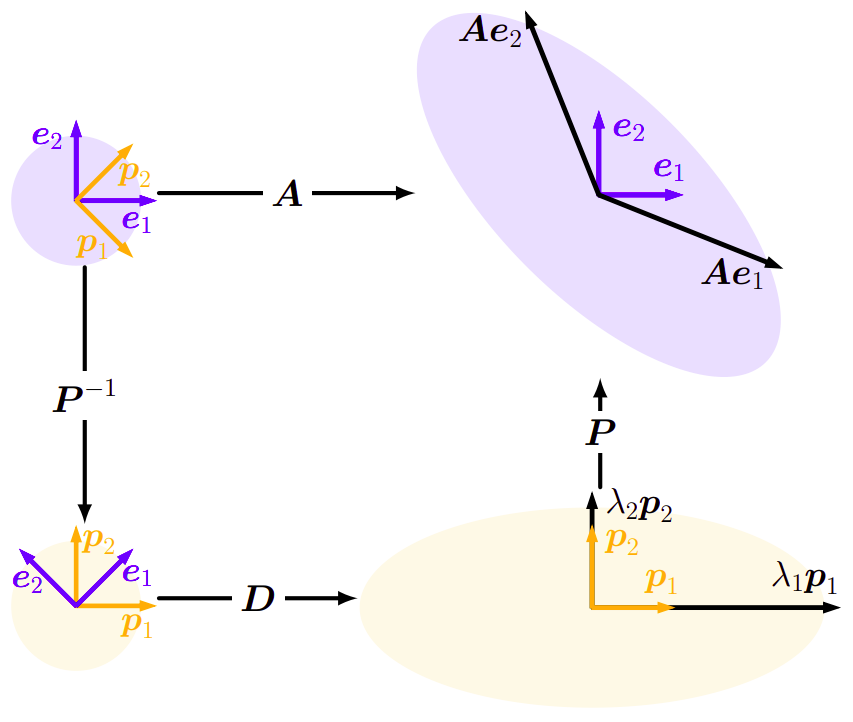
\includegraphics[
        width=\linewidth,
        height=5cm,
        keepaspectratio,
    ]{images/maths-for-ml/eigendecomposition.png}
    \caption*{
        Intuition behind the eigendecomposition as sequential transformations.
        \\
        \textbf{Top-left to bottom-left}: $\bm{P}^{-1}$ performs a basis change (here drawn in $\mathbb{R}^2$ and depicted as a rotation-like operation) from the standard basis into the eigenbasis.
        \\
        \textbf{Bottom-left to bottom-right}: $\bm{D}$ performs a scaling along the remapped orthogonal eigenvectors, depicted here by a circle being stretched to an ellipse. 
        \\
        \textbf{Bottom-right to top-right}: $\bm{P}$ undoes the basis change (depicted as a reverse rotation) and restores the original coordinate frame.
    }
\end{figure}


\begin{enumerate}
    \item 
    \begin{theorem}[Eigendecomposition]
        A square matrix $\bm{A} \in \mathbb{R}^{n\times n}$ can be factored into $\bm{A} = \bm{PDP}^{-1}$ where $\bm{P} \in \mathbb{R}^{n\times n}$ and $\bm{D}$ is a diagonal matrix whose diagonal entries are the eigenvalues of $\bm{A}$, if and only if the eigenvectors of $\bm{A}$ form a basis of $\mathbb{R}^n$.
        \hfill \cite{mfml/book/mml/Deisenroth-Faisal-Ong}
    \end{theorem}
\end{enumerate}








